\section{\Large PROBLEM SET 6}
\subsection{PROBLEM 1}
\textit{Complete the modeling and verification of perturbation torques as described in the previous pset}

We have implemented models of the drag, gravity gradient, magnetic field, and solar radiation pressure effects on our satellite. Please see the relevant portions of the previous section for more detail.


\subsection{PROBLEM 2}
\textit{Compute the attitude control error even if a controller is not implemented yet. The attitude control error represents the rotation between the desired and actual attitude. Plot the attitude control error and give its interpretation. Note that this step requires the definition and computation of the desired or nominal or target attitude of the spacecraft. In general, this can be expressed in body or principal axes.}

Given that the goal of the satellite is to have an Earth-pointing antenna, the ideal position for the satellite is to have the principal z-axis facing the negative radial direction. Additionally, to maximize solar coverage the principal y-axis should be aligned with the normal direction. Because of this, the desired attitude of the spacecraft should simply be the negative of the RTN frame, as shown below. Additionally, the satellite was assumed to be traveling at the mean motion to preserve its Earth-pointing behavior.

\begin{align*}
    \Vec{P}_{desired} &= 
    \begin{bmatrix}
    -1 & 0 & 0 \\
    0 & 0 & 1 \\
    0 & 1 & 1
    \end{bmatrix}
    \Vec{P}_{RTN}
\end{align*}

For the sake of this analysis, the simulated orbit was assumed to start off in the ideal attitude and was assumed to have no torques. Figure \ref{fig:Images/ps6_problem2.png} shows the results of this analysis. Besides some numerical errors, the ideal and simulated attitudes are at the same point, which is expected given the lack of perturbations.

\begin{figure}[H]
\centering
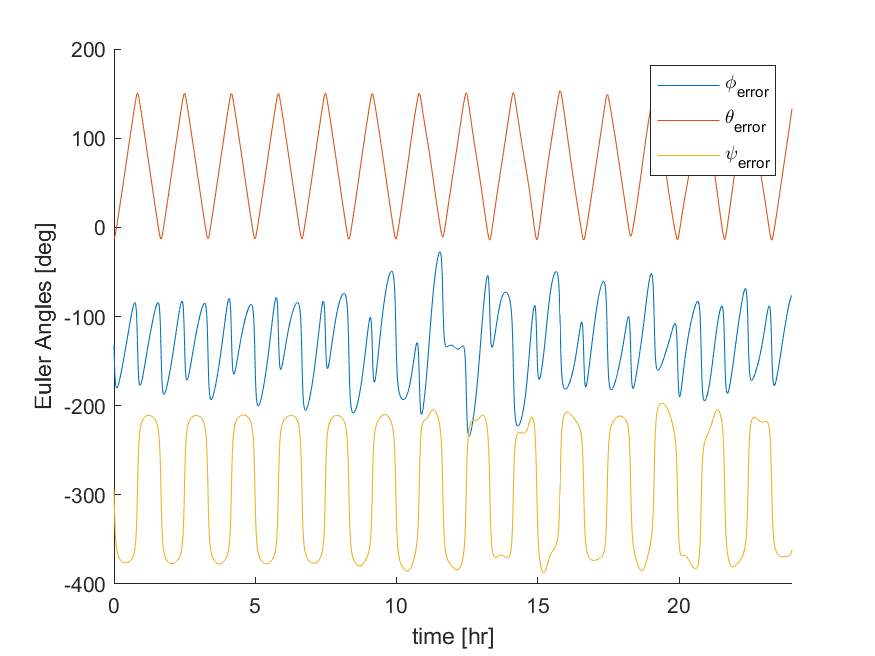
\includegraphics[scale=0.6]{Images/ps6_problem2.png}
\caption{Error between ideal and simulated attitude without perturbations}
\label{fig:Images/ps6_problem2.png}
\end{figure}

\subsection{PROBLEM 3}
\textit{Note that the attitude control error represents a rotation matrix (DCM) which quantifies how far the actual attitude is from the true attitude. You can use any parameterization to plot the attitude control errors corresponding to this DCM. Give interpretation of the attitude control errors given the applied disturbances.}

Show error with perturbation

\subsection{PROBLEM 4}
\textit{You can now start modeling the Simulink spacecraft subsystem which is what the satellite believes is happening (on-board). Initially, the sensors provide ideal measurements (no bias or noise). Just use an empty box for those. The outputs of the sensors are measurements which are used for attitude determination. These measurements are computed from the reference truth or oracle.}

\subsection{PROBLEM 5}
\textit{Assume a certain set of sensors. In general, a number of unit vectors and angular velocities can be considered as measurements}

\textit{Implement the deterministic attitude determination algorithm discussed in class and its variant which uses fictitious measurements to spread the errors across the measurements}

\textit{Implement the statistical attitude determination algorithm discussed in class (q-method)}

\textit{Implement angular velocity measurements and the reconstruction of the attitude from those (through kinematic equations coded identically to ground truth but replicated in the spacecraft on-board computer)}

\subsection{PROBLEM 6}
\textit{Plot the resulting estimated attitude in the absence of sensor errors. Show that it is identical to the true attitude (except for numerical errors).}